\documentclass{article}
\bibliographystyle{IEEEtran}
\usepackage[utf8x]{inputenc}
\usepackage{gensymb}
\usepackage{graphicx}
\usepackage[acronym]{glossaries}
\usepackage{booktabs}
\newcommand{\tabitem}{~~\llap{\textbullet}~~}
\graphicspath{{Images/}}
\usepackage[english]{babel}
\usepackage{natbib}
\usepackage{url}
\usepackage{enumitem}
\usepackage{parskip}
\usepackage{fancyhdr}
\usepackage{amsmath}
\usepackage{vmargin}
\usepackage{indentfirst}
\setmarginsrb{3 cm}{2.5 cm}{3 cm}{2.5 cm}{1 cm}{1.5 cm}{1 cm}{1.5 cm}

\title{Problem Identification, Research, and Requirements Specification Report - Group 23}
\author{}
\date{12 Oct 2018}  

\makeatletter
\let\thetitle\@title
\let\thedate\@date
\makeatother

\makeglossaries
\newacronym{IoT}{IoT}{Internet of Things}
\newacronym{BLE}{BLE}{Bluetooth Low Energy}
\newacronym{API}{API}{Application Programming Interface}
\newacronym{HVAC}{HVAC}{Heating, ventilation, and air conditioning}
\newacronym{ISO}{ISO}{International Organization of Standardization}
\newacronym{SRS}{SRS}{System Requirements Specifications}
\newacronym{UI}{UI}{User Interface}
\newacronym{ML}{ML}{Machine Learning}
\newacronym{DTP}{DTP}{Data Transmission Protocol}
\newacronym{OCS}{OCS}{Occupation Classification System}
\newacronym{AI}{AI}{Artificial Intelligence}

\pagestyle{fancy}
\fancyhf{}
\rhead{\theauthor}
\lhead{\thetitle}
\cfoot{\thepage}

\begin{document}


%%%%%%%%%%%TITLE PAGE%%%%%%%%%%%%%%%%%%%%%%%

\begin{titlepage}
    \centering
    
\includegraphics[scale = 1.48]{UOIT.png}
    \textsc{\LARGE ENG4940 Capstone I \\ Problem Identification, Research, and Requirements Specification Report}
	\rule{\linewidth}{0.2 mm}
	{ \huge \bfseries
	   Environment Sensing\\ Occupancy Integration System\newline}
	\rule{\linewidth}{0.2 mm} \\[1.5 cm]
    
    
    
    \begin{minipage}{0.4\textwidth}
		\begin{flushleft} \large
			\emph{Name:}\\
			Raven Castaneda\\
			Eric Dube\\
			Brady Ibanez\\
            Taylor Somann\\
        
			\end{flushleft}
			\end{minipage}~
			\begin{minipage}{0.4\textwidth}
            
			\begin{flushright} \large
			\emph{Student  Number :} \\
			100559932\\
            100555757\\
            100367230\\
            100502392\\
		\end{flushright}
        
	\end{minipage}\\[2 cm]
    
\end{titlepage}
%%%%%%%%%%%TABLE OF CONTENTS%%%%%%%%%%%%%%
\tableofcontents
\pagebreak
\listoftables
\pagebreak
\listoffigures
\pagebreak
\printglossary[type=\acronymtype,title={List of Abbreviations}]
\pagebreak
%%%%%%%%%%%%%%%%%%%%%%%CONTENT%%%%%%%%%%%%%%%%%%%%%%%%%%
\section{Problem Identification}
\setlength{\parindent}{1cm} It is the intention of this capstone project to allow for the configuration and implementation of an environment detecting \gls{IoT} system. The system will be capable of referencing the environment in which it resides and provide diagnostic feedback to the detailing of specific objects and states that are of particular concern to the situational maintenance it is meant to satisfy. In specific, as a paired grouping capstone project, this system is to be inherently concerned with temperature and humidity detailing, as to allow for the capacity of machine learning oriented \gls{HVAC} control. However, it is to be primarily concerned with allocating the capacity of occupancy status provisions and be capable of identifying entities to be defined as human occupants within the environment monitored.

By providing the machine capacity of a system to be aware of occupants, and to monitor associated parameters such as occupant location, occupant count, occupant status (in terms of environment stay duration), and so forth, any associated environment control systems will be provided a level of insight to their situational control demeanor beyond any other form of direct user controlled environment systematization. In this regard, systems will be allocated capacity for inferential control beyond adherence to static variable coherence, by being provided a degree of environment understanding to a dynamic extent. 

Therefore the precise measure of the problem this project will seek to satisfy: The issue of dynamic \gls{IoT} system inference as attained through passive user interfacing. By providing the capacity for a system to reference user and occupant detailing dynamically and automatically, the systems ability to infer situational requirements becomes a possibility, and allows for much more involved system design when considering the requirements of users and environments from a consistent input spectrum.  

What should also be defined here is the concept of passive user and environment interfacing. The intended concept here is to relate to system interaction from a completely indirect interaction vantage point. The system itself should be capable of inferring required setting alterations and parameters from constant observation through sensor inference, rather than from direct user input. This is something that does not currently exist in an entirely generalized sense in defined \gls{IoT} devices within the smart home/static indoor environment, but rather within specialized implementation for specific capacity devices.  

While systems to a similar extent exist today, they exist through more limited design, coherence, and manifestation. With this in mind, it can be seen how through existing implementations like Lutron lighting \cite{r1} and Legrand Industrial building control systems \cite{r2}, there are potential solutions for occupancy detection and environmental inference. However, these means facilitate only individual case capacity, and do not accommodate for alternatively influencing factors such as pet detection and maintained occupancy count and diagnostics, among an array of other variables that this project will seek to include and detail.

It is felt that the environmental and situational diagnostics that this system is intended to address are vastly required components for the evolution of \gls{IoT} integration in dynamically intelligent control systems. It is a conceptual component that could benefit not only smart home implementation, but other industries including automotive, health care, and education, should the system be constructed in order to be readily integrate-able and readable by other data requesting manipulating services. 

\pagebreak
%%%%%%%%%%%%%%%%%%%%%%%%%%%%%%%%%%%%%%%%%%%%%%%%%%%%%%%%
\section{Project-related Background and Research Review}

It has been determined through research and observation of existing similar project implementation that the most prudent aspect of concern and understanding would be the implementation of accurate and capable sensor actuation and said sensor integration. This is for the reason that while data manipulation will be a key aspect for the operation of a smart HVAC and occupancy observation system, the more major aspect in terms of \gls{IoT} will be the capacity of said system to realize the physical state of the environment it should govern, and for that realization to be conveyed accordingly.  

\subsection{Wireless Sensor \& Actuator Communication}

For the convenience of the user, it is necessary to have wireless communication for sensors and actuators.
Visible wires are aesthetically unpleasant, while the cost of contracted electrical wiring could add hundreds of dollars to the installation cost. We looked at three different options for wireless communication, and compared them by cost, power consumption, and implementation difficulty. During our research, we discovered there were more factors to consider than we had realized. The three options considered were WiFi, \gls{BLE}, and Xbee.

After our research, we determined all these factors are important for our implementation:
\begin{enumerate}
    \item Low cost
    \item Low energy use
    \item Suitable range from thermostat
    \item More than 20 sensor/actuator nodes
\end{enumerate}

WiFi requires inexpensive hardware, with some modules available for as little as seven dollars \cite{r11}. However, there were some major drawbacks which made us consider other options. WiFi is known to have high power consumption. The high range capability and complicated protocol stack contribute to this. WiFi is also designed on Internet protocols, which may not be suitable for high-throughput applications such as sensors.

\gls{BLE} has low power consumption and similar range (20-30 meters) to classic Bluetooth. \gls{BLE} modules are priced similar to WiFi Modules. Like WiFi, \gls{BLE} also uses a star network topology, which makes routing simple in situations where nodes become disconnected, but also limiting range \cite{r13}. One major drawback is that most Bluetooth transceivers support a very small number of simultaneous links (less than 10).

Xbee modules are more expensive than either WiFi or Bluetooth modules, with prices near \$25 per module \cite{r12}, as well as higher energy consumption than \gls{BLE} from our research. Xbee modules have two major advantages over \gls{BLE}: More simultaneous links, and high range (starting at 90 meters). Xbee also uses a mesh topology, which means the range isn't limited to the location of the hub, but also re-routing when devices loose connection takes longer.
\pagebreak

\begin{flushleft}
\large
\addcontentsline{lot}{table}{Wireless Communication Medium Comparisons}
\textbf{Wireless Communication Medium Comparisons}
\end{flushleft}

\begin{tabular}{| c || c | c | c | c | c |}
    \hline
    Device & Cost & Power Consumption & Range & Topology & Link Limit \\
    \hline
    \hline
    WiFi & Cheap & High & ~90m & Star & Many \\
    \gls{BLE} & Cheap & Low & ~30m & Star & Less than 10 \\
    Xbee & More expensive & Medium & ~90m & Mesh & Many \\
    \hline
\end{tabular}

After discussing these data, it was decided to implement both BLE and Xbee transceivers for prototyping, which will allow the collection of experimental data for later defined use cases. This will also necessitate a prototype for a hybridized communication model for sensors and actuators - something that is believed will improve marketability of the real product.

\subsection{Similar Existing Devices}

As far as existing implementation stands, there exists a few resembling capable similarities. For HVAC control, it can be assumed that Thermostat control provides a similar means of environment control as to what has been proposed here. This is seen in devices like the NEST thermostat, and specifically, the NEST temperature sensor \cite{r16}. Simmilarly, the EcoBee thermostat can be seen to apply \gls{ML} and \gls{AI} environment inference and control for \gls{HVAC} systems \cite{r17}. 

Further, a system that exists to a similar extent in providing occupancy detection, but not involved with the same environment monitoring as would be implied in a residence or commercially viable environment, is the TruCount high occupancy vehicle compliance system \cite{r14}. 

The TruCount system acts in order to detect the occupancy count of active mobile vehicles in order to discover whether or not any scanned vehicle is adhering to valid rider count designation. This is done through the utilization of near infrared camera scanning with rendered images processed by image recognition software in order to count the occupancy of the active vehicle scanned. This is the manifestation of most occupancy detection systems; as an \gls{OCS} for vehicles.

In terms of a system that works to detect occupancy within a static environment, such as a residence or a commercial outlet, there exists most prominently proposed system configuration. This is seen definitely in the article 'IoT-based occupancy detection system in indoor residential environments', where it proposed that observed and analyzed dust patterns allow the detection of occupants \cite{r15}.  

However, these aforementioned products and proposals do not implement a means of fluid occupancy and environment detection similar to the extent of what is to be provided through this system. In contrast to others researched, this system will be capable of full and dynamic environment detection and maintenance. The goal will be to infer temperature, humidity, and occupancy detection at any given point of a given constructed environment, and thus convey the given active status of the environment statically and continuously. 

\pagebreak
%%%%%%%%%%%%%%%%%%%%%%%%%%%%%%%%%%%%%%%%%%%%%%%%%%%%%%%%%%
\section{Design Process}

The design process for this project will be Kanban based on the Agile methodology. The Trello web application will be used to produce a distributed Kanban board for the tracking of task priority, progress and the responsible project member. Continuous delivery of tasks and team member communication will be emphasized and recorded. A single task flow will be utilized, moving tasks up and down the defined design process as is appropriate, completing one task at a time (as individuals, sub-teams or in group entirety, as is required) and will iterate through the design process until the task is complete unless it is determined that the task has been mis-prioritized and should be reintroduced into the Kanban priority queue. Although the Kanban methodology is superficially similar to the Scrum methodology, it does not include any of the formalized roles involved in the latter. Instead, tasks will be categorized according to the areas of contribution identified later in this document.

This project will include six major sections. They are hardware design, hardware development, software design, software development, software integration and software testing. As this is an IoT project, the hardware necessary to run the system must be designed and developed. In order to determine hardware requirements, a (System Requirement Specification) document as defined in Section \gls{ISO} 29148.9.4.15 System Life Cycle Sustainment will be generated. Sections 9.4.16 Packaging, Handling, Shipping and Transportation will be excluded as these subsections deal with logistical and manufacturing concerns which will not be a consideration for this project. This will be used to inform a survey and analysis of available sensors, communication modules, single board computers, micro-controllers and RF communication protocols. Once decisions have been made on each of the required components, the overall hardware system will be designed. Based on the determinations made during system design, multiple devices will need to be produced. These include the sensor units, actuation units and hub-thermostat. We are currently operating under the assumption that the thermostat application, hub application and machine learning model developed by the ML team will run on a single piece of hardware, although this may be subject to change.

In order to properly design the necessary software components, the team will perform a requirements analysis based on stakeholder requirements outlined in this document. We will generate a \gls{SRS}, as per \gls{ISO} 29148.9.5, as the basis for all other software design and development tasks. Although the design and development of the main system will be given priority, the team will also develop mobile and web applications for interacting with the system depending on time constraints. For this project, a HestiaPi open source thermostat design will be implemented. The systems to be designed and developed are as followed:

\begin{flushleft}
\large
\addcontentsline{lot}{table}{Required Included Systems}
\textbf{Required Included Systems}
\end{flushleft}
\begin{itemize}
    \item{Data Management System}
	\item{Data Transit Protocol}
	\item{Hub Application}
	\item{Sensor Software}
	\item{Actuation Software}
	\item{Touch Interface and Web Application}
	\item{Mobile Application}
\end{itemize}

For development of this application, the team will be using a test-driven development strategy. This will require team members to produce unit tests which correspond to a requirement outlined in the \gls{SRS} before beginning development of a feature or application and developing the application until the test can be passed. The developer will then produce another unit test corresponding to a different requirement and continue development for this test case until all requirements are met. This will act as an executable requirement, expressing the functionality of the resulting code and the system as a whole in a set of verifiable, business language requirements.

Once development, and therefore unit testing, has been completed, integration will commence. As the \gls{DTP} (Data Transit Protocol) is a requirement for both the \gls{ML} and \gls{IoT} team, its integration with the Hub application will be given priority. Each integration will be performed with the central application of the system, the Hub. System integration will be required, each with its own subsequent integration testing phase.


\begin{flushleft}
\large
\addcontentsline{lot}{table}{Integration Components}
\textbf{Integration Components}
\end{flushleft}
\begin{itemize}
	\item{HestiaPi Thermostat Integration}
	\item{Data Transit Protocol Integration}
	\item{Sensor Software Integration}
	\item{Actuation Software Integration}
	\item{Web Application Integration}
	\item{Mobile Application Integration}
\end{itemize}

Once integration and the associated testing has been completed, it will be ready for system testing. Testing will commence with the localized system comprised of the applications developed by the \gls{IoT} team, not including the web application or mobile application. Once the local systems has been verified and validated, we will perform integration and system testing with the ML team and the web/mobile applications, if time permits their development. Once both teams are fully integrated, final system testing will commence and be completed.
\\
\hphantom{xx}
\begin{flushleft}
\large
\addcontentsline{lof}{figure}{Team Member Responsibilities}
\textbf{Team Member Responsibilities}
\small
\\
\hphantom{xx}
Raven C.: Sensor unit hardware design and development, sensor software

Taylor S.: Project management, Hub application design and development

Brady I.: Sensor software, circuit design

Eric D.: Middleware and communication design and development
\end{flushleft}
\pagebreak
%%%%%%%%%%%%%%%%%%%%%%%%%%%%%%%%%%%%%%%%%%%%%%%%%%%%%%%%%%
\section{Use Cases and Scenarios}

Defined below is a consideration of active use cases that provide visualization of user interaction with the system. These cases provide a means of understanding and accounting for expected user interaction with the system, and provide a means of adapting functionality from automatic perception and execution.

\begin{flushleft}
\textbf{Use Case 1}

Name: User changes average temperature of room

Description: The User changes the average temperature of the overall system.

Preconditions:
User either has access to the Hub-Stat or access to the system via wireless connections

Post-conditions: N/A

Course of Action:
\end{flushleft}
\begin{enumerate}[noitemsep,nolistsep]
    \item User accesses the hub.
    \item System displays main page.
    \item User selects "Current Target Temperature" Tab.
    \item System updates \gls{UI} to Temperature Screen.
    \item User inputs new temperature setting.
    \item System reads temperature setting and prompts a confirmation.
    \item User confirms the changes.
    \item System acclimates the temperature range accordingly.
\end{enumerate}

\begin{flushleft}
Alternate Course A: User accesses hub via wireless login
\end{flushleft}
\begin{enumerate}[noitemsep,nolistsep]
    \item A.1. User accesses the hub login.
    \item A.2. User inputs user name and password.
    \item A.3. System verifies user name and password.
    \item A.4. Use case continues at course of action step 2.
\end{enumerate}
\begin{flushleft}
Alternate Course B: User declines changes
\end{flushleft}
\begin{enumerate}[noitemsep,nolistsep]
    \item B.7. User declines the changes.
    \item B.8. System reverts current \gls{UI} to Temperature Screen.
    \item B.9. User changes temperature.
    \item B.10. Use case continues at course of action step 6.
\end{enumerate}
\begin{flushleft}
\textbf{Use Case 2}

Name: User Enters and is static (sleeping or idle) in room.

Description: The user enters the room, temperature adjusts based on his entry and maintained based on presence or eventual lack of presence.

Preconditions:

User enters room through traditional means. An example of an nontraditional mean is climbing in a window.

Post-conditions:

User's current location in the room or exiting the room.

Course of Action:
\end{flushleft}
\begin{enumerate}[noitemsep,nolistsep]
    \item User enters room of measure.
    \item Sensor detects user's entry.
    \item Sensors communicate with Hub.
    \item Hub factors in current ambient temperatures with temperature changing variables such as insulation.
    \item The system acclimates for a person staying in the room after a buffer period to confirm occupancy.
    \item User is finished being static in the room, and proceeds to exit room of measure.
    \item Sensor detects user's exit.
    \item Sensors communicate with Hub.
    \item Hub factors in change of heat signature and adjusts accordingly.
\end{enumerate}

\begin{flushleft}
    Alternate Course A: User leaves before buffer period is finished.
\end{flushleft}
\begin{enumerate}[noitemsep,nolistsep]
    \item A.6. User decides to exit room of measure.
    \item A.7. Sensors detects user's exit.
    \item A.8. Sensors communicate with Hub.
    \item A.9. System does not apply any temperature changes, as occupancy was not long enough to justify adjustment.
\end{enumerate}

\begin{flushleft}
\textbf{Use Case 3}

Name: User is hosting a social gathering.

Description: The User is hosting a social gathering and multiple heat signatures will be entering and leaving at different intervals.

Preconditions:
User and guests enters room through traditional means and measuring from a residential doorway. An example of an nontraditional mean is climbing in a window.

Post-conditions: N/A

Course of Action:
\end{flushleft}
\begin{enumerate}[noitemsep,nolistsep]
    \item People enter the doorway in different intervals.
    \item Sensors detects the amount of people entering.
    \item Sensors communicate with Hub.
    \item System calculates the amount of acclimation needed to achieve temperature of user's choice.
    \item After buffer period, system begins adjusting settings for temperature.
    \item Sensors detect people exiting.
    \item Sensors communicate with Hub.
    \item System adjusts based on amount of people leaving.
\end{enumerate}

\begin{flushleft}
Alternate Course A: Users leave before buffer period ends.
\end{flushleft}
\begin{enumerate}[noitemsep,nolistsep]
    \item A.5. Heat signatures leave before buffer period is over.
    \item A.6. Sensors detect heat signatures exiting.
    \item A.7. Sensors communicate with Hub.
    \item A.8. System acclimates for amount of people leaving.
    \item A.9. Use case continues at course of action step 5.
\end{enumerate}

\pagebreak


%%%%%%%%%%%%%%%%%%%%%%%%%%%%%%%%%%%%%%%%%%%%%%%%%%%%%%%%%%
\section{Stakeholder Requirements}
Primary stakeholders of this project from the direct perspective of residential environment automation include residents and occupants of the system integrating environment. This includes occupying home owners and tenants. These stakeholders must be considered primary for the fact that they will be the most involved and effected individuals in respect to system interaction and control. The operation of the system and it's purpose entirely revolve around the capacity it maintains to benefit the comfort and convenience of these stakeholders on a daily basis.  

These stakeholders require the fulfillment of reliably accurate environment and occupancy detection, analysis, and detailing. From the environmental aspect, it is necessary for the system to include readings of temperature and humidity. A deviation in temperature within 1.0 degree Celsius is shown to have no impact on thermal comfort\cite{r4}. Furthermore, from further research, it has been found that temperature readings should not exceed a deviated value of greater or less than 0.5 degrees Celsius to prevent noticeable temperature deviation without active intervention\cite{r3}. This standpoint has been taken to adhere to a greater caution factor in system quality maintenance. From the occupancy detection aspect, there will need to be a means of qualifying registered system users (who have inputted as known entities to the system) from general occupants. There should be a 95 percent accurate value provided for general occupant count to compensate for misinterpreted signals confusing human numbers, and a 70 percent accurate value for readings of registered users. 

It is furthermore crucial that an aspect of system activity timing be implemented as to ensure a smooth and cohesive interaction between users and the system. In this sense, it is thus necessary to include minimum response and delivery times while within the confines that must be adhered to, in order for the system to pass this requirement. 

One aspect that must be restrained by timing confines is the capacity for direct user interaction with the system (the hub in particular or alternative control interface in particular) to edit temperature settings. With this in mind, users should be able to input an alteration to thermostat settings and receive immediate acceptance and integration of the changes to system variables and parameters. This will result in immediate \gls{HVAC} response, profile edits, and scheduling requests.

This leads to the next timing related requirement; scheduling capacity. Primary stakeholders will be provided the ability to request scheduling alterations. This implies the ability to implement alterations that will take effect at a requested time will occur will be made available by the capacity of the system to infer timing mechanism.

Another main concern and requirement that must be facilitated for these stakeholders is the factor of privacy and anonymity. Due to the design of the system, it will require the capacity to interface with other potential users to augment functionality capabilities, including potential homestead administrators and third party product developers. Crucial user details (especially registered user details) should never be shared or made vulnerable to other stakeholder system interaction.

Further primary stakeholders who are not subject to first person interaction with the active system include individuals involved in the maintenance and construction of system controlled environments. Such stakeholders consist of non-occupying home owners, residential property administrators, as well as property developers and constructors. These stakeholders, while not experiencing direct effect of the system during active operation, are subject to effects in terms of either existing system status diagnostics and/or system implementation. 

It is necessary that these stakeholders be aware of both proper system installation practices, as well as system failures. This first item is important for the reason that without an appropriate means of installation, either facilitated by themselves or a third party installer, it can not be assumed that system integration will allow for proper operation, and thus will result in inaccurate and faulty operation. These stakeholders will also require information concerning any faulty operation within a system that might occur after installation for the reason of vested interest in both the system installed, as well as the residence in which the system is operating. In particular, faulty temperature readings alternative to expected reading values can be indicative of a malfunctioning \gls{HVAC} system, which could lead to residence damage. These notifications must be free of fault and inaccuracy such that false alarms be avoided entirely.

Developers of the configuration and creation of the system are primary stakeholders as well. Their requirements involve the assurance of system reliability and operability, which is defined and guaranteed through initial testing practices outlined in the Project Plan section. 

Secondary stakeholders include third party developers who may come to deal with integration of the system as a subsystem within other systems they create themselves. Requirements in this regard entail the ability to interact with sensor read values of the environment. This then leads to the requirement of available sensor interpreted readings, since these stakeholders will require the insight of the system primarily as a means of elevating the implementation of their own systems. In order to achieve this, it will be necessary that the means of sensor interpretation be provided through a central location connected to the internet. This location will require security authentication, meaning third party stakeholders should not be able to access an operating instance of the system without authentication satisfaction as constructed by registered user acceptance. This can be done through the creation of a public \gls{API} allowing third party developers the ability to write general functionality for the system they do not have access to, until a system user provides it.  

The one requirement to maintain above others is that of privacy for direct system interactors. This is for the fact that the requirements of all non direct interactors with the system will require access to some capacity, but that the provisioning of this access could compromise direct users who will be exposing much more sensitive personal information. It is for this reason that the satisfaction of another requirement will have to be reconsidered should it compromise the occupant's system security and privacy requirement.  

Refer to the table provided below for a concise summary of the identified stake holders and their corresponding requirements. Note that requirements will be defined with an identifying variable reference (ex. R1 for the first identified requirement) for use in later sections:
\pagebreak

\begin{flushleft}
\large
\addcontentsline{lot}{table}{Stakeholder Requirements}
\textbf{Stakeholder Requirements}
\end{flushleft}

\begin{center}
\begin{tabular}{lll}
\hline Customers & Primary & \tabitem R1: 95\% accurate occupancy detection \\
 & & \tabitem R2: 70\% accurate registered user detection\\
 & & \tabitem R3: Non-deviant temp readings greater or less\\ 
 & & \hphantom{xx} than 0.5\degree C \\ 
 & & \tabitem R4: System occupancy count reliability \\
 & & \tabitem R5: System security, and privacy \\ 
 & & \tabitem R6: The ability to accept third party product \\ 
 & & \hphantom{xx} interaction requests \\ 
 & & \tabitem R7: The immediate implementation of direct \\ 
 & & \hphantom{xx} user alterations \\
 & & \tabitem R8: Scheduling capability \\ \hline
 Administrators & Primary & \tabitem R9: Installation documentation and references\\
 and Developers& & \tabitem R10: Accurate system failure notification \\ \hline
 Third-Party & Secondary & \tabitem R11: A public \gls{API} for auxiliary product \\ 
 Developers & & \hphantom{xx} creation \\
 & & \\ 
 & & \\ 
 & & \\
\end{tabular}
\end{center}

\pagebreak
%%%%%%%%%%%%%%%%%%%%%%%%%%%%%%%%%%%%%%%%%%%%%%%%%%%%%%%%%
\section{Definition of Acceptance Tests}
Since it is the intention of this project to implement hardware and software interfacing, it will be necessary to include testing designed for both included hardware to correctly and accurately reference the environment aspects intended to be characterized, as well as for software configuration to be able to accurately respond to the hardware provided data sets. For the purpose of detailing these tests in this section, hardware testing will be acknowledged first. 

This system will be primarily concerned with referencing linear, instantaneous capturing of environment data. As such, the hardware will need to provide static references throughout elapsed time. This is intended for the most part in order to reduce processing capacity requirements within sensors, and will also help to reduce the detail required in hardware testing. In this way, sensors will merely have to be tested for singular event accuracy. 

For temperature sensor (thermometer) testing, analog reference of a given temperature within an environment will be initially taken. Simultaneous reference provided by the configured thermometer sensor will be compared. A passing value from the sensor will adhere to a deviation of recorded temperature no greater or less than 0.5 degrees Celsius compared to the analog thermometer. A similar testing protocol will be adhered to for humidity testing in reference to relative humidity. 

For occupancy testing, the test practice parameters will adhere similarly to those mentioned above, where comparative measures are provided merely through first person human recordings. The sensor must be able to detect human presences with 95\% accuracy to achieve a passing value. Occupancy sensors must also be able to detect registered users and provide a Boolean reference variable value asserting the registration status of the user. The existence and accuracy of this variable must be referenced during testing and correlate to the perceived status of the recorded occupant. Hardware testing only needs to correlate to sensor accuracy for the static variables for which they provide representation.

In reference to software testing, a perspective concerning a recorded comparison schema must be most prudently adhered to and maintained. It should be the active ability of the data set configuring software component (the thermostat/hub) to allow for data maintenance and manipulation from the sensors to illustrate a workable set. In terms of temperature, software inference of the environmental data points provided by the sensors should be manifested as a table of points correlating to the time at which they were attained. For this reason, it must be possible to confirm temperature and humidity data update times within a set period. Updates must be attained accurately within 5 minutes intervals and reflect appropriately the temperatures and humidity recorded at those times. The five minute interval was determined for temperature reading particularly for being in adherence to the time span utilized in a 2016 study of occupant thermal comfort \cite{r5}

In terms of occupancy referencing by software, updates must be provided per noticed alteration per sensor. For this reason, continuous reading would be ideal, however, to save processor capacity and usage within sensors, it is instead decided that update intervals can expand to the 5 second range. This can be the case for all sensors except for occupancy volume sensors at residence entry and exit points which cannot afford any delay. This would be to prevent inaccurate current live occupancy for the entire environment monitored by the system. In order to test this, variable values for overall occupancy and individual space occupancy must be maintained and referenced in comparison to physically perceived values.

Since software implementation cannot wait for hardware implementation prior to functionality testing, it has been decided as well that simulation testing must also play a role in ensuring sound software operation. Thus a corresponding simulation test for each hardware correlated test will also be conducted prior to hardware integrated testing practices. Simulation must generate random values of registered user variable with predefined profiles as well to test appropriate integration of registered user object profiles.

Security testing will be included and executed through a means of active affirmation through attempts made by requesting third-party interfaces to access sensitive data. A passing test will be attained when it is confirmed that sensitive data is not viable through the \gls{API}. 

Refer to the table provided below for a concise summary of the intended acceptance tests to be conducted. Note that acceptance tests will be defined with an identifying variable reference (ex. T1 for the first test) for use in later sections:

\begin{flushleft}
\large
\addcontentsline{lot}{table}{Acceptance Tests}
\textbf{Acceptance Tests}
\end{flushleft}

\begin{center}
\begin{tabular}{ll}
\hline
 \textbf{Test Name} & \textbf{Description}  \\ \hline
 T1 \hphantom{x}- Confirm temperature reading & Ensure that sensor reading correlates within \pm 0.5^{\circ}C $ \\ 
 & of analog reading.\\
 T2 \hphantom{x}- Confirm humidity reading & Ensure that sensor reading correlates within 5\% \\ 
  & relative humidity analog reading.\\ 
 T3 \hphantom{x}- Detect non-registered users & Ensure human occupancy detection within 95\% \\
 & accuracy.\\
 T4 \hphantom{x}- Detect registered users & Ensure registered user occupancy with 70\% accuracy\\
 T5 \hphantom{x}- Confirm temperature relay & Ensure hub component receives temperature reading\\
 & from sensor at 5 minute intervals.\\
 T6 \hphantom{x}- Confirm humidity relay & Ensure hub component receives humidity reading from\\
 & sensor at 5 minute intervals.\\
 T7 \hphantom{x}- Confirm human detection & Ensure hub component receives occupant count++ \\
 \hphantom{xxxx} (non-entry point sensor) & accurately within 5 seconds of change.\\
 T8 \hphantom{x}- Confirm human detection & Ensure hub component receives occupant count++\\
 \hphantom{xxxx} (entry point sensor) & accurately within 1 second of change.\\
 T9 \hphantom{x}- Simulate T7 & Used solely for application functionality confirmation.\\
 T10 - Simulate T8 & Used solely for application functionality confirmation.\\
 T11 - Confirm registered user detection & Ensure system is capable of registered user recognition \\
 & in practice.\\
 T12 - Simulate registered occupant & Randomly assign registered user Boolean variable in\\
 & same testing format as T9 and T10 once successfully\\
 & completed.\\
 T13 - Confirm security integrity & Attempt to access data through API implementation \\
 T14 - Confirm input received from hub & Attempt to make alterations through hub interface\\
 & considering schedule alterations.
\end{tabular}
\end{center}


\pagebreak
%%%%%%%%%%%%%%%%%%%%%%%%%%%%%%%%%%%%%%%%%%%%%%%%%%%%%%%%%
\section{Traceability Matrix}
This traceability matrix illustrates a means for gauging stakeholder requirement satisfaction. It is believed that through the completion of the defined acceptance tests that an idea of the extent of satisfaction of the requirements will be provided. The following matrix outlines which tests will satisfy acceptable performance of the systems ability to maintain the requirement referenced:

\begin{flushleft}
\large
\addcontentsline{lof}{figure}{Traceability Matrix}
\textbf{Traceability Matrix}
\end{flushleft}

\begin{center}
\begin{tabular}{|l|l|l|l|l|l|l|l|l|l|l|l|l|l|}
\hline
 \textbf{Requirements} & ||| & \textbf{R1} & \textbf{R2}  & \textbf{R3} & \textbf{R4} & \textbf{R5} & \textbf{R6}  & \textbf{R7} & \textbf{R8} & \textbf{R9} & \textbf{R10} & \textbf{R11}\\ \hline
 \textbf{Test Cases} & \textbf{Totals}& 5 & 3 & 2 & 8 & 1 & 2 & 6 & 3 & 0 & 1 & 1\\ \hline
 \textbf{T1}  &  3  &     &     &  X  &     &     &  X  & X    &  &  &  &\\ \hline
 \textbf{T2}  &  1  &     &     &     &     &     &    &  X   &  &  &  & \\ \hline
 \textbf{T3}  &  2  &  X  &     &     &  X  &     &     &     &  &  &  & \\ \hline
 \textbf{T4}  &  2  &     &  X  &     &  X  &     &     &     &  &  &  &  \\ \hline
 \textbf{T5}  &  3  &     &     &  X  &     &     &    &   X     &  X  &  &  &  \\ \hline
 \textbf{T6}  &  2  &     &     &     &     &     &    &  X   & X  &  &  & \\ \hline
 \textbf{T7}  &  2  &  X  &     &     &  X  &     &     &     &  &  &  & \\ \hline
 \textbf{T8}  &  2  &  X  &     &     &  X  &     &     &     &  &  &  & \\ \hline
 \textbf{T9}  &  2  &  X  &     &     &  X  &     &     &     &  &  &  &  \\ \hline
 \textbf{T10} &  2  &  X  &     &     &  X  &     &     &     &  &  &  &   \\ \hline
 \textbf{T11} &  2  &     &  X  &     &  X  &     &     &     &  &  &  &  \\ \hline
 \textbf{T12} &  2  &     &  X  &     &  X  &     &     &     &  &  &  &  \\ \hline
 \textbf{T13} &  5  &     &     &     &     &  X  &  X  &  X  &   &   &  X  &  X \\ \hline
 \textbf{T14} &  2  &     &     &     &     &     &     &  X  &  X  &    &    &  \\ \hline
\end{tabular}
\end{center}

It is acknowledged that no current acceptance test exists for the installation documentation and references requirement within the traceability matrix. That has been considered, and should it be deemed necessary, it could be completed through customer user surveying. This is for the fact that it will be a necessary outcome of first hand installation experience that will help provide necessary detail for creation. 

It should also be noted that while it is realized that some tests do not facilitate required testing consideration in entirety for certain requirements, they will still contribute aspects of confirmation if they are selected to correlate.  

\pagebreak
%%%%%%%%%%%%%%%%%%%%%%%%%%%%%%%%%%%%%%%%%%%%%%%%%%%%%%%%%%%%
\section{Project Plan}

A project Gantt chart has been generated, outlining each major task in the Design Process, with estimates of time required to complete said task. Given the expected timeline, the Hub Application should be completed mid-November, in time to begin integration of the different modules. This will allow us to fulfill the requirements of Report 2 and should result in a viable prototype. Integration with the Machine Learning team may not be fully completed at this time, but the device should be capable of performing each function necessary to fulfill the conceptual design.

If the project does not progress as predicted, the implementation of certain features outside of the core functionality of the project may be deferred to the winter semester.


\begin{flushleft}
\large
\addcontentsline{lof}{figure}{Gantt Chart}
\textbf{Project Gantt Chart}
\end{flushleft}

\begin{flushleft}
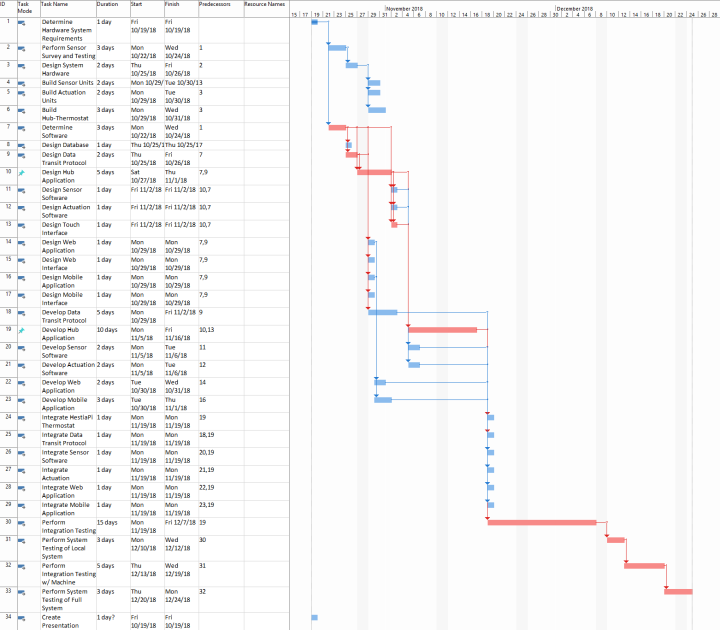
\includegraphics[scale = .6]{Gantt.png}
\end{flushleft}

\pagebreak
%%%%%%%%%%%%%%%%%%%%%%%%%%%%%%%%%%%%%%%%%%%%%%%%%%%%%%%%%%%%
\section{Contribution Matrix}

While contribution detailing does not require strict adherence in the sense that any given contribution head may not apply effort outside of their given effort set, the following work concentration divide means to provide governance of developer focus within the project.

\begin{flushleft}
\textbf{Raven C. -- Head of Sensors, Research Assistant, Sensor Software Assistant, Report Assistant}
\end{flushleft}

Raven will be responsible for designing and implementing the sensors for the system, as well as provide research support and sensor software assistance.

\begin{flushleft}
\textbf{Taylor S. -- Project Manager, Hub Designer, Head of Software}
\end{flushleft}

Taylor will be responsible for heading the project, keeping the project on time, and designing the main hub for the system.

\begin{flushleft}
\textbf{Brady I. -- Head of Sensor Software, Head of Report Organization, Circuit Designer}
\end{flushleft}

Brady will be responsible for the implementation and synchronization of \gls{BLE} sensor integration to allow for the capacity of the system to infer physical recognition of the environment governed.

\begin{flushleft}
\textbf{Eric D. -- Head of Middleware, Head of Research}
	Eric will be responsible for
\end{flushleft}
\end{flushleft}

\pagebreak
%%%%%%%%%%%%%%%%%%%%%%%%%%%%%%%%%%%%%%%%%%%%%%%%%%%%%%%%%%%%
\newpage
\bibliographystyle{plain}
\bibliography{biblist}
\hphantom{\cite{r6}}
\hphantom{\cite{r7}}
\hphantom{\cite{r8}}
\hphantom{\cite{r9}}
\hphantom{\cite{r10}}

\end{document}

%%%%%%%%%%%%%%%%%%%%%%%%%%%%%%%%%%%%%%%%%%%%%%%%%%%%%%%%%%%%%
